
\documentclass{CLS_zhou430}

% Additional Packages
\usepackage{subcaption}
\usepackage{booktabs}
\usepackage{multirow}



\newcommand{\projecttitle}{Aircraft Maintenance Anomaly Detection System}
\addauthor{Pratima Rajbanshi}{w10161681}{Computer Science}
\addauthor{Samarpan Thapa}{w10163103}{Computer Science}



%%%%%%%%%%%%%%%
%% Starting your report
%%%%%%%%%%%%%%%

\begin{document}
\frontmatter

%%%%%%%%%%%%%%%
%%% Modify as needed
%%%%%%%%%%%%%%%

\begin{abstract}
The project proposes the development of a system for anomaly detection and Remaining Useful Life (RUL) prediction for landing gear sensor data of aircraft. Six different anomaly detection algorithms, namely, Z-Score, Isolation Forest, K-Mean, DBSCAN, One-Class SVM, and LSTM Autoencoders, are implemented for six different synthetic Airbus datasets, consisting of 278,000 data points. An interactive dashboard using the Streamlit library facilitates the results for the maintenance crew. So far, the implementation of all the anomaly detection algorithms and the dashboard have been completed. Preliminary results indicate the feasibility of the Isolation Forest algorithm. Further, cross-validation of the results over different datasets, tuning of the parameters, and testing of the results remain to be done.
\end{abstract}


\begin{acknowledgments}
We would like to thank Dr.\ Zhaoxian Zhou for his guidance throughout the project and UWE Bristol for their publicly available synthetic landing gear datasets. We would also like to thank the University of Southern Mississippi School of Computing Sciences and Computer Engineering for providing the resources to complete this capstone.
\end{acknowledgments}

%%%%%%%%%%%%%%%%%%%%%%%%%%%%%
%%%%%%%%%%%%%%%%%%%%%%%%%%%%%
\makelists


%%%%%%%%%%%%%%%%%%%%%%%%%%%%%
%%%%%%%%%%%%%%%%%%%%%%%%%%%%%
\chapter{Introduction} \label{chap:intro}

The current state of aircraft maintenance involves massive amounts of data from various sensors. Scheduled maintenance reduce the occurrence of failures, but early signs of failures, e.g., minor pressure changes, temperature surges, or slow degradation, are hidden amongst thousands of other noises and very hard to identify by human beings. \cite{carvalho2019systematic, chandola2009anomaly}. This project proposes the application of data-driven anomaly detection and RUL estimation for synthetic landing gear sensor data, highlighting the role of machine learning as a supporting system. \cite{ran2019survey}.

\section{Background}
The landing gear system on an airplane is a safety-critical system that endures tremendous mechanical stress under flight conditions such as takeoff and landing \cite{do2004proactive}. With the use of data analytics, predictive maintenance can be achieved to avoid failures before they happen \cite{compare2020challenges}. However, there is a lack of publicly available data for landing gear. So, this project usees the synthetic datasets provided by UWE Bristol \cite{uwe2023landing}, which are based on real Airbus data and created with GANs \cite{goodfellow2014generative}.

\section{Problem Statement}
The data related to aircraft maintenance is highly voluminous, complex, and distributed over time. The current techniques are unable to detect small changes that often occur prior to the degradation of the equipment. The present project aims to develop an automatic system that can analyze the landing gear sensor data and identify abnormal patterns, yet be understandable to maintenance personnel.

\section{Project Objectives}
\begin{enumerate}
    \item Implement and compare six anomaly detection algorithms on landing gear time-series data.
    \item Develop an RUL estimation module for components exhibiting gradual degradation.
    \item Build an interactive dashboard for data exploration, parameter configuration, and anomaly inspection.
    \item Evaluate each method's detection rate and computational performance across six datasets.
\end{enumerate}

\section{Scope}
\textbf{In scope:} Six synthetic CSV datasets; six anomaly detection methods; RUL estimation; Streamlit dashboard; method comparison.

\textbf{Out of scope:} Real-time streaming; integration with aircraft maintenance management systems; autonomous decision-making.


%%%%%%%%%%%%%%%%%%%%%%%%%%%%%
%%%%%%%%%%%%%%%%%%%%%%%%%%%%%
\chapter{Literature Review}

\section{Overview of Related Work}
A detailed taxonomy of anomaly detection methodologies is given in Chandola et al.\ \cite{chandola2009anomaly}. The most promising approaches are ensemble methods and deep learning for predictive maintenance, as indicated in Carvalho et al.\ \cite{carvalho2019systematic}. The most popular RUL dataset used in research is the NASA C-MAPSS dataset\ \cite{saxena2008damage}. However, it only considers landing gear failure in engines. The linear degradation model is still effective for sensors with a monotonous trend, as indicated in Si et al.\ \cite{si2011remaining}.

\section{Previous Approaches}
\textbf{Statistical Methods} (Z-Score) enable fast anomaly flagging but assume normality and ignore multivariate dependencies \cite{chandola2009anomaly}. \textbf{Isolation Forest} \cite{liu2008isolation} uses anomaly isolation based on random partitioning, where the computational complexity is linear. \textbf{K-Means} and \textbf{DBSCAN} \cite{ester1996density} use clustering for anomaly detection, where the number of clusters is not required for DBSCAN. \textbf{One-Class SVM} \cite{scholkopf2001estimating} learns a boundary around normal data but is computationally expensive. \textbf{LSTM Autoencoders} \cite{malhotra2016lstm} reconstruct normal sequences and flag high-error sequences as anomalous, capturing temporal dependencies that point-level methods miss \cite{hochreiter1997long}.

\section{Gaps and Relevance}
The gaps in the existing research include the scarcity of landing gear-related data, the absence of comparative studies using multiple methods, the lack of interpretability of the results in deep learning models, and the absence of user-centric tools. \cite{uwe2023landing}. This project attempts to bridge all four gaps by comparing six methods on the same landing gear datasets and developing an interactive dashboard. We use scikit-learn \cite{pedregosa2011scikit} and TensorFlow \cite{tensorflow2015} as implementation frameworks.


%%%%%%%%%%%%%%%%%%%%%%%%%%%%%
%%%%%%%%%%%%%%%%%%%%%%%%%%%%%
\chapter{Engineering Standards}

\section{Industry Standards}
The current project is based on \textbf{IEEE/ISO/IEC 12207} \cite{ieee12207} standards for software life cycle processes and \textbf{IEEE/ISO/IEC 29148} \cite{ieee29148} for requirements engineering. The code is written in accordance with PEP 8 guidelines and uses type hints and modular design. It is also version-controlled using Git.

\section{Compliance and Safety}
The datasets are used under Creative Commons licenses with proper attribution to UWE Bristol. The system is clearly designed to be a decision support tool, detecting anomalies and highlighting them, but not taking any maintenance actions. It does this to follow aviation industry standards. There are multiple methods to detect anomalies with variable thresholds, which can be adjusted to suit the user’s needs, along with transparency in the dashboard.


%%%%%%%%%%%%%%%%%%%%%%%%%%%%%
%%%%%%%%%%%%%%%%%%%%%%%%%%%%%
\chapter{System Design and Methodology}

\section{System Overview}
The system is a Python-based analytics pipeline with four components: (1) data ingestion and preprocessing, (2) anomaly detection algorithms, (3) RUL estimation, and (4) an interactive visualization dashboard. Figure~\ref{fig:arch} shows the architecture.

\begin{figure}[h]
    \centering
    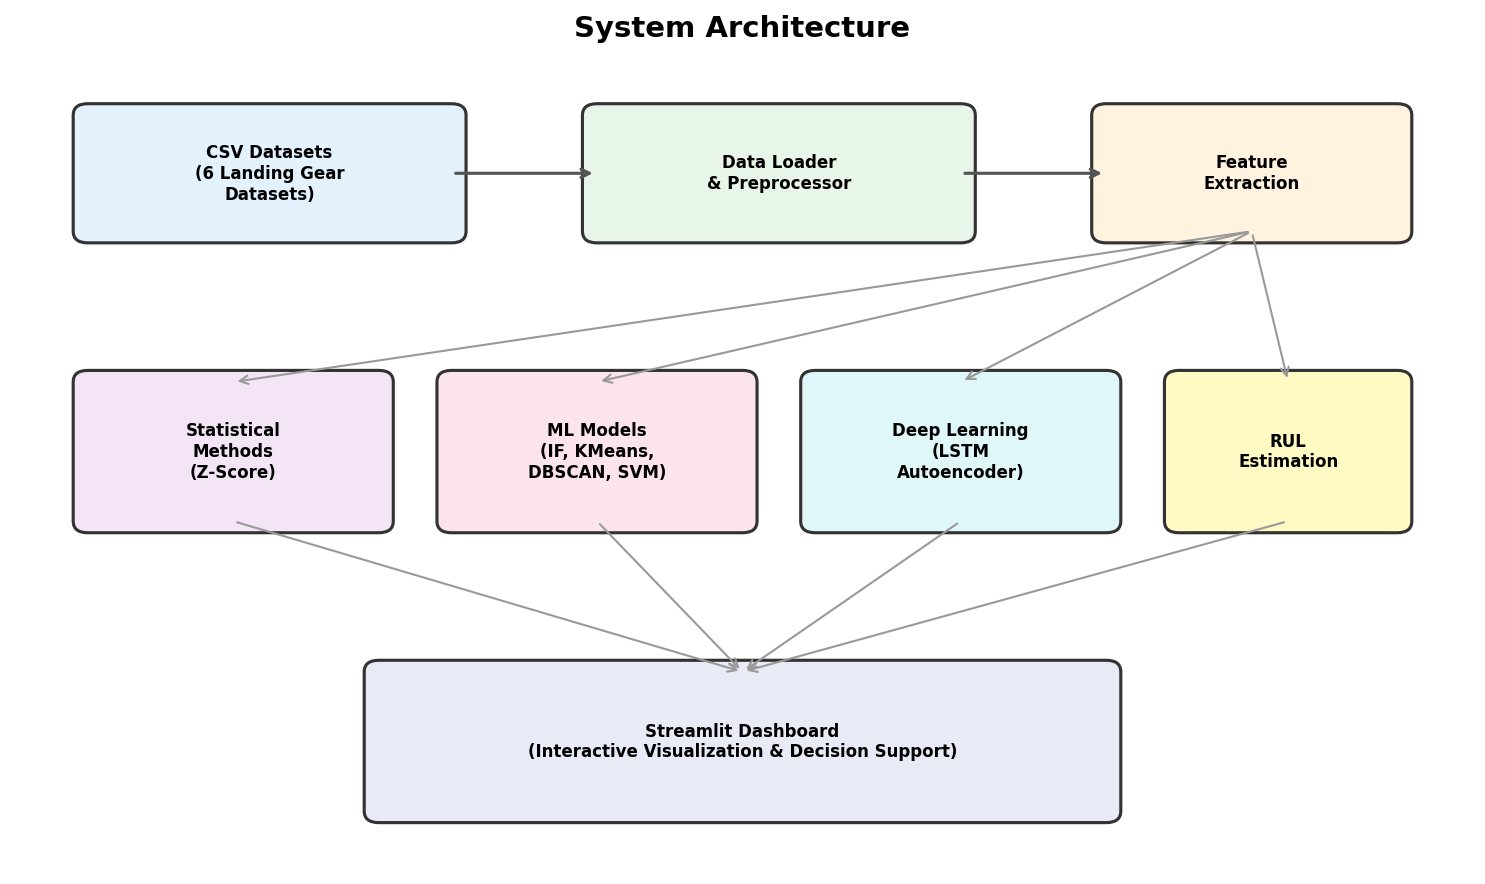
\includegraphics[width=0.9\textwidth]{figs/fig_architecture.png}
    \caption{System Architecture}
    \label{fig:arch}
\end{figure}

\section{Software Architecture and Tools}
The software consists of four Python modules: \texttt{data\_loader.py} (CSV loading, normalization, statistics), \texttt{anomaly\_detection.py} (five detection methods plus RUL), \texttt{autoencoder.py} (LSTM encoder-decoder), and \texttt{visualization.py} (Plotly charts). The Streamlit dashboard (\texttt{app.py}) integrates all modules into five pages: Overview, Data Explorer, RUL Estimation, Anomaly Detection, and LSTM Autoencoder.

Key technologies: Python 3.13, pandas/NumPy, scikit-learn \cite{pedregosa2011scikit} (Isolation Forest, K-Means, DBSCAN, One-Class SVM), TensorFlow/Keras \cite{tensorflow2015} (LSTM Autoencoder), SciPy, Plotly, and Streamlit.

\section{Development Methodology}
Development followed three iterative phases: (1) data exploration and summary statistics, (2) modular algorithm implementation with configurable parameters, and (3) dashboard integration with Streamlit caching for performance.

\section{System Flow}
The user can choose a dataset and method through the sidebar. The data loader will return a pandas DataFrame, the detection algorithm will add \texttt{is\_anomaly} flags, and the visualization module will render interactive charts. For RUL estimation, linear regression will extrapolate degradation trends to critical thresholds.


%%%%%%%%%%%%%%%%%%%%%%%%%%%%%
%%%%%%%%%%%%%%%%%%%%%%%%%%%%%
\chapter{Design Constraints}

\section{Technical Constraints}
The synthetic datasets may not capture the failure modes present in the real world. There are no ground truth anomaly labels available, so supervised learning is not feasible. There are six datasets, ranging from 20,000 to 108,000 rows, and 2 to 24 sensors. Therefore, the methods must generalize well for different dimensionalities. 

\section{Resource and Performance Constraints}
The project is using open-source tools, and the license cost for these tools is zero. These tools are being executed on consumer-grade hardware, and the size of the deep learning model must be limited. Therefore, the methods must execute the datasets in a matter of seconds. Z-Score takes less than 0.01 s, and Isolation Forest takes 0.56 s, whereas DBSCAN takes 11.98 s and One-Class SVM takes 13.45 s. Therefore, these two algorithms qualify for the project, whereas the other two algorithms are slow. Since the project is using the Streamlit framework, the data loading would be cached, so there would be no redundancy. 

\section{Trade-offs}
The project needs to consider the following trade-offs: speed and accuracy, simplicity and power, sensitivity and specificity. Z-Score is the fastest but only detects extreme univariate outliers. Isolation Forest is fast and captures multivariate anomalies. K-Means and DBSCAN can capture complex patterns but are slower and require parameter tuning. One-Class SVM is powerful but computationally expensive. LSTM Autoencoders can capture temporal dependencies but require more data and tuning.


%%%%%%%%%%%%%%%%%%%%%%%%%%%%%
%%%%%%%%%%%%%%%%%%%%%%%%%%%%%
\chapter{Implementation Progress}

\section{Completed Work}
The program consists of about 600 lines of Python code in four modules. The \texttt{data\_loader.py} module loads all six datasets, extracts the sensor columns, normalizes the features, and calculates the statistics. The \texttt{anomaly\_detection.py} module includes the implementation of the Z-Score method, Isolation Forest, K-Means, DBSCAN, and One-Class SVM algorithms, as well as the RUL estimation using linear extrapolation. The \texttt{autoencoder.py} module includes the implementation of the autoencoder algorithm using a two-layer LSTM encoder-decoder architecture that detects anomalies based on the reconstruction error. The \texttt{visualization.py} module provides six different types of Plotly charts. The program is connected with the Streamlit dashboard.

\section{Challenges}
The challenges encountered in the project include the variety of the datasets, which makes the program require flexible code for different sizes and names of the columns. The DBSCAN algorithm is extremely sensitive to the choice of the parameter epsilon. The training time of the LSTM autoencoder is relatively long. The inability to compute precision/recall without ground-truth labels.


%%%%%%%%%%%%%%%%%%%%%%%%%%%%%
%%%%%%%%%%%%%%%%%%%%%%%%%%%%%
\chapter{Preliminary Results}

\section{Anomaly Detection Performance}
We compare the performance of the methods using the detection rate, computation time, and qualitative assessment of the domain. Table~\ref{tab:metrics} shows the results for the methods on Dataset 1.

\begin{table}[h]
    \centering
    \caption{Anomaly Detection Performance (Dataset 1: Bogie Pitch Trimmer, 40,000 rows, 8 sensors).}
    \begin{tabular}{|l|c|c|c|}
        \hline \hline
        Method & Anomalies & Rate (\%) & Time (s) \\ \hline
        Z-Score ($\theta=3.0$) & 1,327 & 3.32 & 0.01 \\ \hline
        Isolation Forest ($c=0.05$) & 2,000 & 5.00 & 0.56 \\ \hline
        K-Means ($k=3$, $p=95$) & 2,000 & 5.00 & 2.16 \\ \hline
        DBSCAN ($\varepsilon=1.5$, $m=10$) & 4 & 0.01 & 11.98 \\ \hline
        One-Class SVM ($\nu=0.05$) & 2,000 & 5.00 & 13.45 \\ \hline
        \hline
    \end{tabular}
    \label{tab:metrics}
\end{table}

\section{Observations}
The best trade-off of detection quality (5\%) and efficiency (0.56s) is achieved by the Isolation Forest algorithm. The Z-Score method is the fastest (0.01s) but detects only extreme univariate outliers (3.32\%). The DBSCAN method detects only 4 points, and hence its parameters need to be tuned for the given data. The One-Class SVM method performs as well as the Isolation Forest method but is 24 times slower. These observations are consistent with the expectations based on the literature \cite{liu2008isolation, ester1996density, scholkopf2001estimating}. Figure~\ref{fig:comparison} and Figure~\ref{fig:timeseries} show the method comparison and the sample detection results.

\begin{figure}[h]
    \centering
    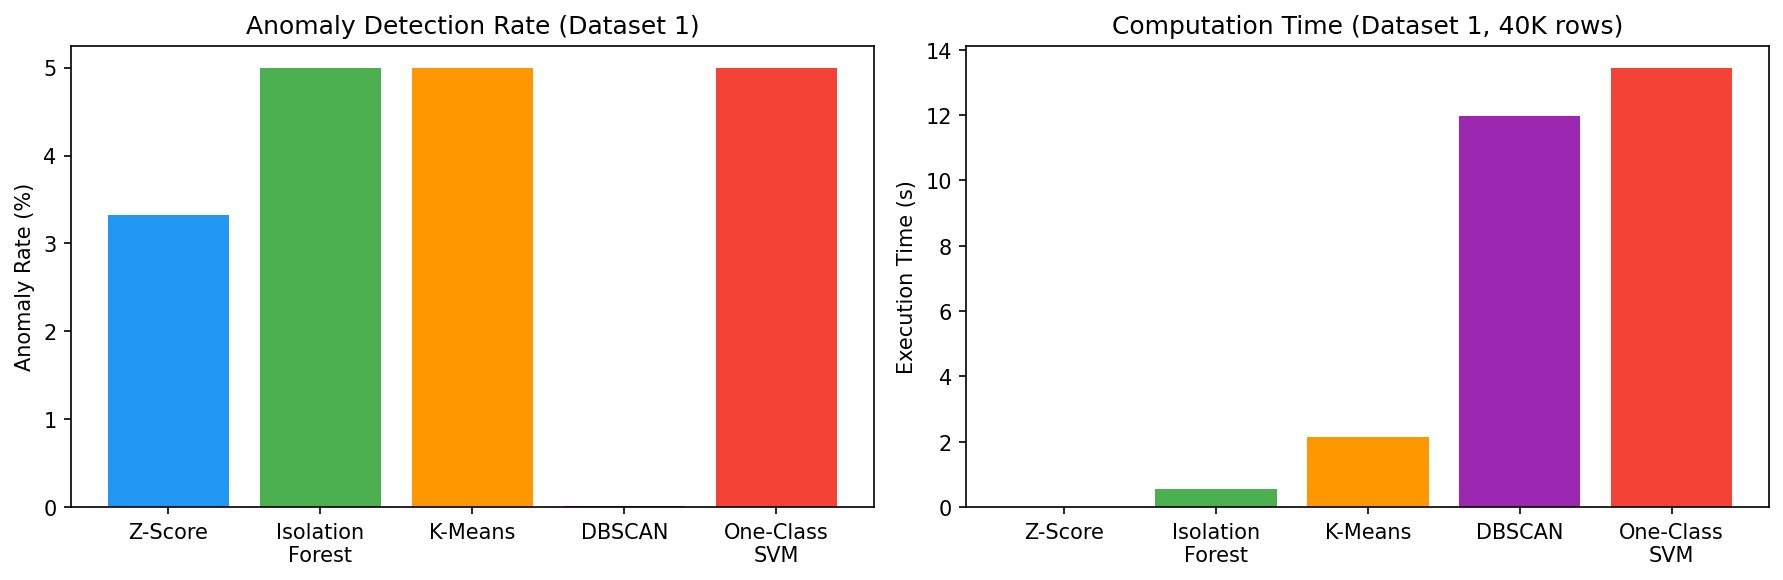
\includegraphics[width=0.95\textwidth]{figs/fig_method_comparison.png}
    \caption{Detection Rate and Computation Time Comparison (Dataset 1)}
    \label{fig:comparison}
\end{figure}

\begin{figure}[h]
    \centering
    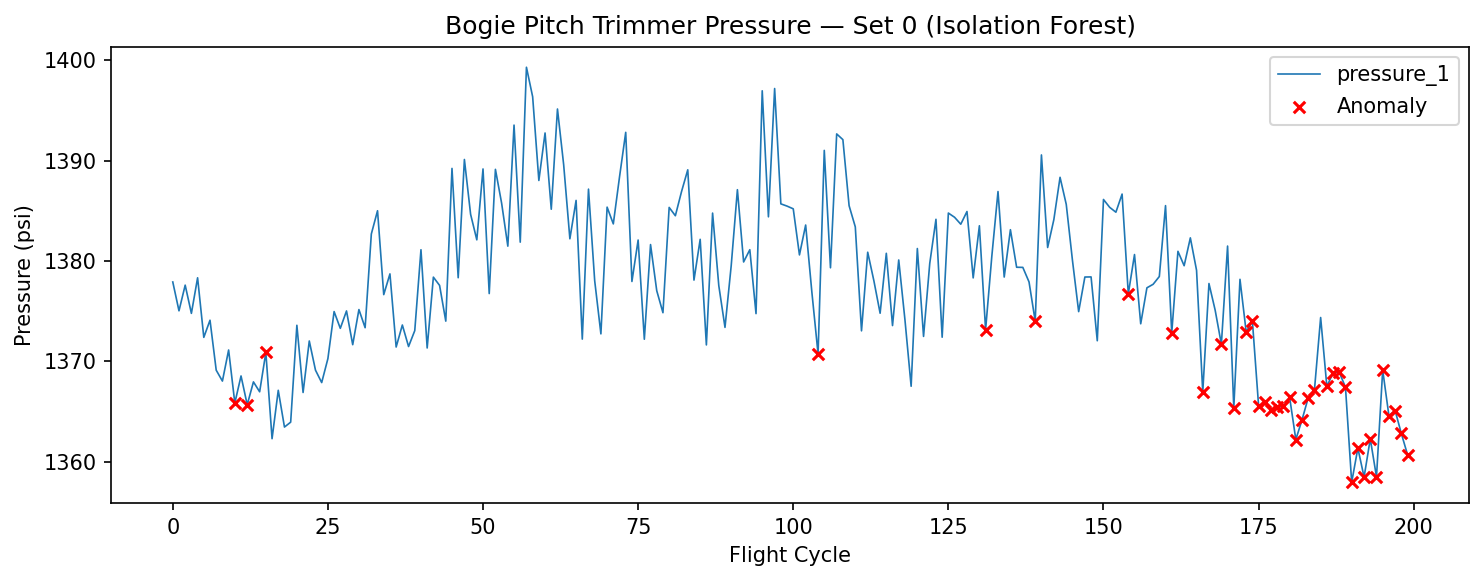
\includegraphics[width=0.95\textwidth]{figs/fig_timeseries_anomaly.png}
    \caption{Bogie Pitch Trimmer Pressure with Isolation Forest Anomaly Detection (Set 0)}
    \label{fig:timeseries}
\end{figure}


%%%%%%%%%%%%%%%%%%%%%%%%%%%%%
%%%%%%%%%%%%%%%%%%%%%%%%%%%%%
\chapter{Current Status and Remaining Work}

\section{Current Status}
The following tasks are completed as of the midterm:
- Loading and validation of all six datasets.
- Implementation of five-point level detection algorithms.
- LSTM autoencoder is working with the default hyperparameters.
- RUL estimation is functional across all six datasets.
- Streamlit dashboard is operational.
- Preliminary comparison on Dataset 1 is complete.

\section{Remaining Work}
\begin{enumerate}
    \item Cross-dataset evaluation across all six datasets.
    \item LSTM Autoencoder hyperparameter tuning.
    \item DBSCAN automated parameter selection.
    \item RUL validation across more time series.
    \item Dashboard polish and comprehensive testing.
    \item Final report with full analysis and conclusions.
\end{enumerate}

\section{Timeline}
\begin{table}[h]
    \centering
    \caption{Remaining Project Timeline}
    \begin{tabular}{|l|l|}
        \hline \hline
        Week & Tasks \\ \hline
        Week 9--10 & Cross-dataset evaluation, LSTM tuning \\ \hline
        Week 11--12 & DBSCAN optimization, RUL validation \\ \hline
        Week 13--14 & Dashboard polish, comprehensive testing \\ \hline
        Week 15--16 & Final report writing and submission \\ \hline
        \hline
    \end{tabular}
    \label{tab:timeline}
\end{table}



%%%%%%%%%%%%%%%%%%%%%%%%%%%%%
%%%%%%%%%%%%%%%%%%%%%%%%%%%%%
\addcontentsline{toc}{chapter}{Bibliography}
\bibliographystyle{abbrv}
\bibliography{references}


\end{document}
